\documentclass[../cheatSheetAlgoritmi.tex]{subfiles}
\begin{document}

\subsection{Esercitazione 14 - 03/06/20}
\textbf{Sequenza Specchiata}\\
Dato un vettore $V$ di $n$ interi appartenenti all’insieme \{0,1\}, si scriva un algoritmo che restituisca la lunghezza del più lungo sottovettore contiguo formato da $k$ valori 0 seguiti da $k$ valori 1. Si noti che è possibile che esistano altri valori 0 prima del sottovettore così individuato, oppure altri valori 1 dopo il sottovettore, ma non è possibile che si verifichino entrambe le estensioni, altrimenti il sottovettore non sarebbe massimale. Discutere correttezza e complessità dell'algoritmo proposto.\\
Esempio: per l’input 001111111\textbf{000111}10000, l’algoritmo deve restituire 6.\\
\begin{lstlisting}[caption=Sequenza Specchiata]
int mirrored(int[] V, int n)
	int maxValue = 0
	int one = 0
	int zero = 0
	for i = 1 to n do
		if V[i] $==$ 0 then
			one = 0
			zero = zero + 1
		else
			if zero $>$ 0 then
				one = one + 1
				maxValue = max(maxValue, min(zero, one))
			if one > zero or (i < n and V[i+1] $==$ 0) then
				zero = 0
	return 2*maxValue
\end{lstlisting}
L'algoritmo conta le occorrenze di 0 fino a quando non incontra un 1, a quel punto, se il numero di zeri è maggiore di 0, viene preso il valore massimo tra la più grande sequenza specchiata trovata fino ad ora e il minimo tra il numero di 0 e 1 attuale. Nel caso in cui le occorrenze di uno sono maggiori di quelle di zero non è più necessario contare poichè si è già trovata la sequenza massima e bisognerà attendere la prossima sequenza di zeri; nel caso in cui viceversa la sequenza di uno sia più breve di quella di zero allora è necessario ripartire a contare gli zeri. La complessità dell'algoritmo proposto è $\mathcal{O}(n)$.\\\\
\textbf{Aggiornamento del flusso massimo}\\
Sia $G= (V, E, s, t, c)$ una rete di flusso con valori interi. Si supponga di conoscere un flusso massimo in $G$, e si supponga che la capacità di un singolo arco $(u, v) \in E$ sia aumentata di una unità. Progettare un algoritmo per aggiornare il flusso massimo in tempo $\mathcal{O}(n+m)$ oppure $\mathcal{O}(n^{2})$.\\
La soluzione al problema consiste nel modificare la versione dell'algoritmo maxFlow (\emph{Ford-Fulkerson}) presentato nella sezione di \emph{Ricerca Locale} della dispensa. Essendo che tra i vari dati vi è anche il flusso massimo attuale e la funzione di capacità è possibile ricavarsi la capacità residua tramite differenza e il cammino aumentante implementato tramite una visita bfs e una memorizzazione tramite liste di adiacenza.
\begin{lstlisting}[caption=Aggiornamento Flusso Massimo]
int mirrored(int[] V, int n)
	% Rete Residua
	int[][] r = int[1...n][1...n]
	% Cammino Aumentante
	int[][] g = int[1...n][1...n]
	% Aumento di capacita' previsto nel problema 
	c[u][v] = c[u][v] + 1
	r = c - f
	g = cammino-aumentate(r, n, s, p)
	f = f + g
\end{lstlisting}
Visto che le operazioni tra matrici impiegano tempo $\mathcal{O}(n^{2})$ per essere eseguite questo è anche il costo complessivo dell'algoritmo in quanto in un grafo completo con nodi con $n-1$ archi la visita costerebbe comunque $\mathcal{O}(n^{2})$.\\\\
\textbf{Ballo di Fine Anno}\\
Una scuola vuole organizzare un ballo di fine anno. Ci sono $n$ maschi e $m$ femmine. Ogni coppia di studenti (composta da un ragazzo ed una ragazza che intendono danzare insieme) ha dovuto registrarsi (altrimenti non avrebbero potuto danzare insieme). I regolamenti della scuola impongono che ogni coppia non possa danzare insieme più di 3 volte. In più, ogni studente non può danzare più di 10 volte in totale. Potete assumere che il ballo duri abbastanza a lungo da permettere a tutti di completare le proprie danze, se le registrazioni lo permettono.\\
\textbf{Descrivere} un algoritmo che, dato in input l’insieme dei maschi e delle femmine e l’insieme delle registrazioni, massimizzi il numero di danze in totale. Discutere la complessità dell’algoritmo proposto.\\
\textbf{Soluzione:} Il seguente problema può essere risolto mediante la costruzione di una Rete di Flusso $G = (V, E, s, p, c)$
\begin{itemize}
	\item $V$ è l'insieme dei nodi appartenenti alla rete di flusso ed è costruito come segue 
	\begin{itemize}
		\item Aggiungiamo $n$ nodi, uno per ogni ragazzo
		\item Aggiungiamo $m$ nodi uno per ogni ragazza
		\item Aggiungiamo $s$ e $p$ supersorgente e superpozzo 
		\item In totale abbiamo $n + m + 2$ nodi
	\end{itemize}
	\item $E$ è l'insieme degli archi della rete di flusso ed è costruito in questo modo
	\begin{itemize}
		\item Aggiungiamo un arco da $s$ a ogni $n_{i}$ ($1 \leq i \leq n$)
		\item Aggiungiamo un arco $\forall n_{i} \mid 1 \leq i \leq n$ a $m_{j}$ ($ \forall j \mid 1\leq j \leq m$)
		\item Aggiungiamo infine un arco $\forall m_{j} \mid 1 \leq j \leq m$ entrante in $p$
	\end{itemize}
	\item $s$ è definito supersorgente
	\item $p$ è definito superpozzo
	\item $c: V \times V \rightarrow \mathbb{R}$ è chiamata capacità ed è definita come segue
	\begin{itemize}
		\item Associamo agli archi uscenti da $s$ una capacità pari a 10
		\item Associamo agli archi uscenti da $n_{i}$ ($1 \leq i \leq n$) una capacità pari a 3, nel caso in cui la coppia si sia registrata per danzare insieme, altrimenti 0
		\item Associamo agli archi uscenti da ogni $m_{j}$ ($1 \leq j \leq m$) una capacità pari a 10
	\end{itemize}
	\item La complessità dell'algoritmo proposto è pari a $min$(Ford-Fulkerson, Edmonds-Karp) = $min(\mathcal{O}((V + E) \mid f^{*} \mid), \mathcal{O}(VE^{2}))$:
		\begin{itemize}
			\item Il numero di nodi complessivi è dato da $n + m + 2$
			\item Il numero di archi complessivi è dato da $n + nm + m$
			\item Il flusso massimo è pari a $10 \cdot min(n,m)$
			\item Per Ford-Fulkerson il limite superiore dunque è pari a $\mathcal{O}(n^{2-k} m^{1+k})$ con $k = 0$ se $n > m$ mentre $k = 1$ se $m > n$
			\item Per Edmons-Karp il limite superiore è pari a $\mathcal{O}(min(m^{2} n^{3}, m^{3} n^{2}))$
			\item In questo caso la complessità da scegliere è quella data da Ford-Fulkerson\\
		\end{itemize}
\end{itemize}
\begin{figure}[h]
\caption{Rete di Flusso - Ballo Scolastico}
\centering
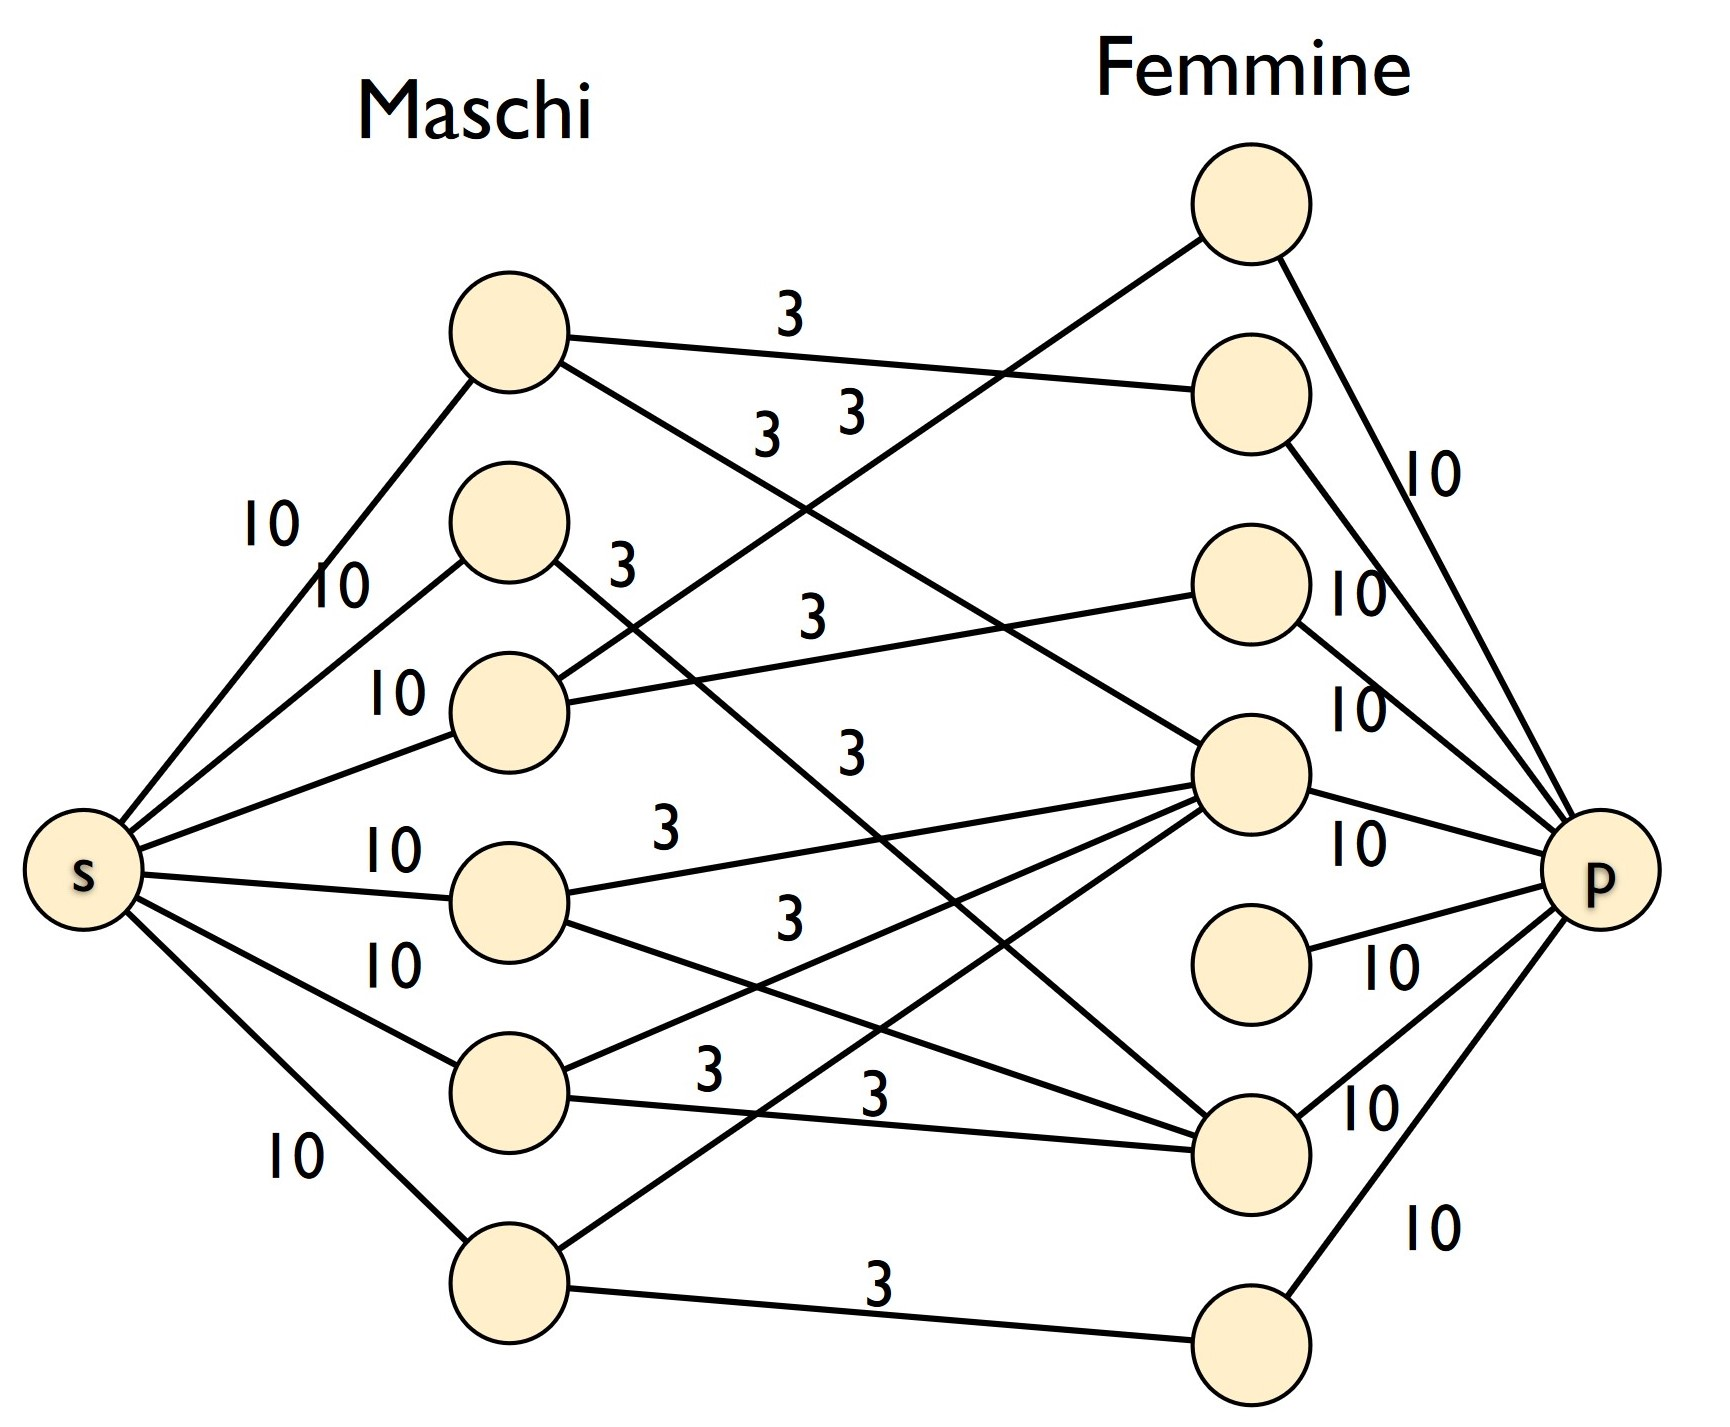
\includegraphics[width=0.5\textwidth]{../img/Locale_4.jpg}
\end{figure}
\textbf{Piscina}\\
Siete responsabile dei corsi di nuoto organizzati da una piscina pubblica. I corsi vengono gestiti settimanalmente. Ogni corso dura un’ora. Ogni corso può avere al massimo 6 bambini. Ogni corso ha un orario di inizio che può andare dalle 9 alle 18 (per un totale di dieci corsi al giorno). Ogni bambino sceglie a quanti corsi partecipare alla settimana, ma questo numero non può essere superiore a 5 e non si può fare lezione più di due volte lo stesso giorno. Poiché i poveri bambini moderni sono stressati da mille altri corsi (calcio, musica, etc), ogni bambino può dare un certo numero di preferenze (ore in cui può partecipare ad un corso). Ogni corso deve essere insegnato da un insegnante. Ogni insegnante può dare un certo numero di disponibilità (ore in cui può insegnare un corso). Infine, ogni bambino che segue un corso paga 10 euro. \textbf{Descrivere} un algoritmo che di assegnamento bambini-corsi-insegnanti che massimizzi il guadagno, descrivendo per bene input, output. Discutere la complessità.\\
\textbf{Soluzione:} Il seguente problema può essere risolto mediante la costruzione di una Rete di Flusso $G = (V, E, s, p, c)$
\begin{itemize}
	\item $V$ è l'insieme dei nodi appartenenti alla rete di flusso ed è costruito come segue 
	\begin{itemize}
		\item Aggiungiamo $b$ nodi, uno per ogni bamino
		\item Aggiungiamo $7b$ nodi, cioè 7 nodi per ogni bambino rappresentanti la sua settimana
		\item Aggiungiamo $70$ nodi, cioè 10 nodi per ogni giorno della settimana rappresentati l'orario a cui può svolgersi il corso il tal giorno
		\item Aggiungiamo $i$ nodi, uno per ogni insegnante
		\item Aggiungiamo un nodo $s$ e $p$ rispettivamente supersorgente e superpozzo
		\item In totale abbiamo $b + 7b + 70 + 70 + 2$ nodi (prevedendo direttamente il caso peggiore in cui il numero di insegnanti sia pari al numero di corsi)
	\end{itemize}
	\item $E$ è l'insieme degli archi della rete di flusso ed è costruito in questo modo
	\begin{itemize}
		\item Aggiungiamo un arco da $s$ a ogni $b_{i}$ con $1 \leq i \leq b$
		\item Aggiungiamo un arco $\forall b_{i} \mid 1 \leq i \leq b$ a $g_{ij}$ ($ \forall j \mid 1\leq j \leq 7$), cioè da bambino ai giorni in cui si tengono i corsi (7 giorni per ogni bambino)
		\item Aggiungiamo un arco $\forall  g_{ij} \mid 1 \leq i \leq b \land 1 \leq j \leq 7$ a $c_{jk}$ ($\forall k \mid 1 \leq k \leq 10$), cioè associamo ogni orario (dalle 9 alle 18) di ogni giorno della settiamana a un corso
		\item Aggiungiamo un arco $\forall  c_{jk} \mid 1 \leq j \leq 7 \land 1 \leq k \leq 10$ all'insegnante $i_{c}$ (!$\exists$ $1 \leq c \leq i \mid i_{c}$ vuole insegnare in quell'orario)
		\item Aggiungiamo infine un arco $\forall i_{c} \mid 1 \leq c \leq i$ entrante in $p$
	\end{itemize}
	\item $s$ è definito supersorgente
	\item $p$ è definito superpozzo
	\item $c: V \times V \rightarrow \mathbb{R}$ è chiamata capacità ed è definita come segue
	\begin{itemize}
		\item Associamo agli archi uscenti da $s$ una capacità pari a 5
		\item Associamo agli archi uscenti da $b_{i}$ ($1 \leq i \leq b$) capacità pari a 2
		\item Associamo agli archi uscenti da $g_{ij}$ ($1 \leq i \leq b$ $\land$ $1 \leq j \leq 7$) capacità 0 nel caso non possa partecipare in quell'ora altrimenti 1
		\item Associamo agli archi uscenti da ogni $c_{jk}$ ($\forall k \mid 1 \leq k \leq 10$) una capacità pari a 6
		\item Associamo una capacità pari a +$\infty$ agli archi entranti in $p$ in quanto non abbiamo vincoli sugli insegnanti
	\end{itemize}
	\item La complessità dell'algoritmo proposto è pari a $min$(Ford-Fulkerson, Edmonds-Karp) = $min(\mathcal{O}((V + E) \mid f^{*} \mid), \mathcal{O}(VE^{2}))$:
		\begin{itemize}
			\item Il numero di nodi complessivi è dato da $b + 7b + 70 + 70 + 2 = 8b + 142$
			\item Il numero di archi complessivi è dato da $b + 7b + 70b + 70 + 70 = 78b + 140$
			\item Il flusso massimo è pari a $5b$ e viene limitato dal fatto che è possibile al massimo fare 10 corsi al giorno per ogni giorno della settimana con 6 bambini ognuno
			\item Per Ford-Fulkerson il limite superiore dunque è pari a $\mathcal{O}(b^{2})$
			\item Per Edmons-Karp il limite superiore è pari a $\mathcal{O}(b^{3})$
			\item In questo caso la complessità da scegliere è quella data da Ford-Fulkerson\\
		\end{itemize}
		\item Il guadagno massimo settimanale è dunque $6 \times 10 \times 7 \times 10 = 4200$\\
\end{itemize}
\begin{figure}[h]
\caption{Rete di Flusso - Piscina}
\centering
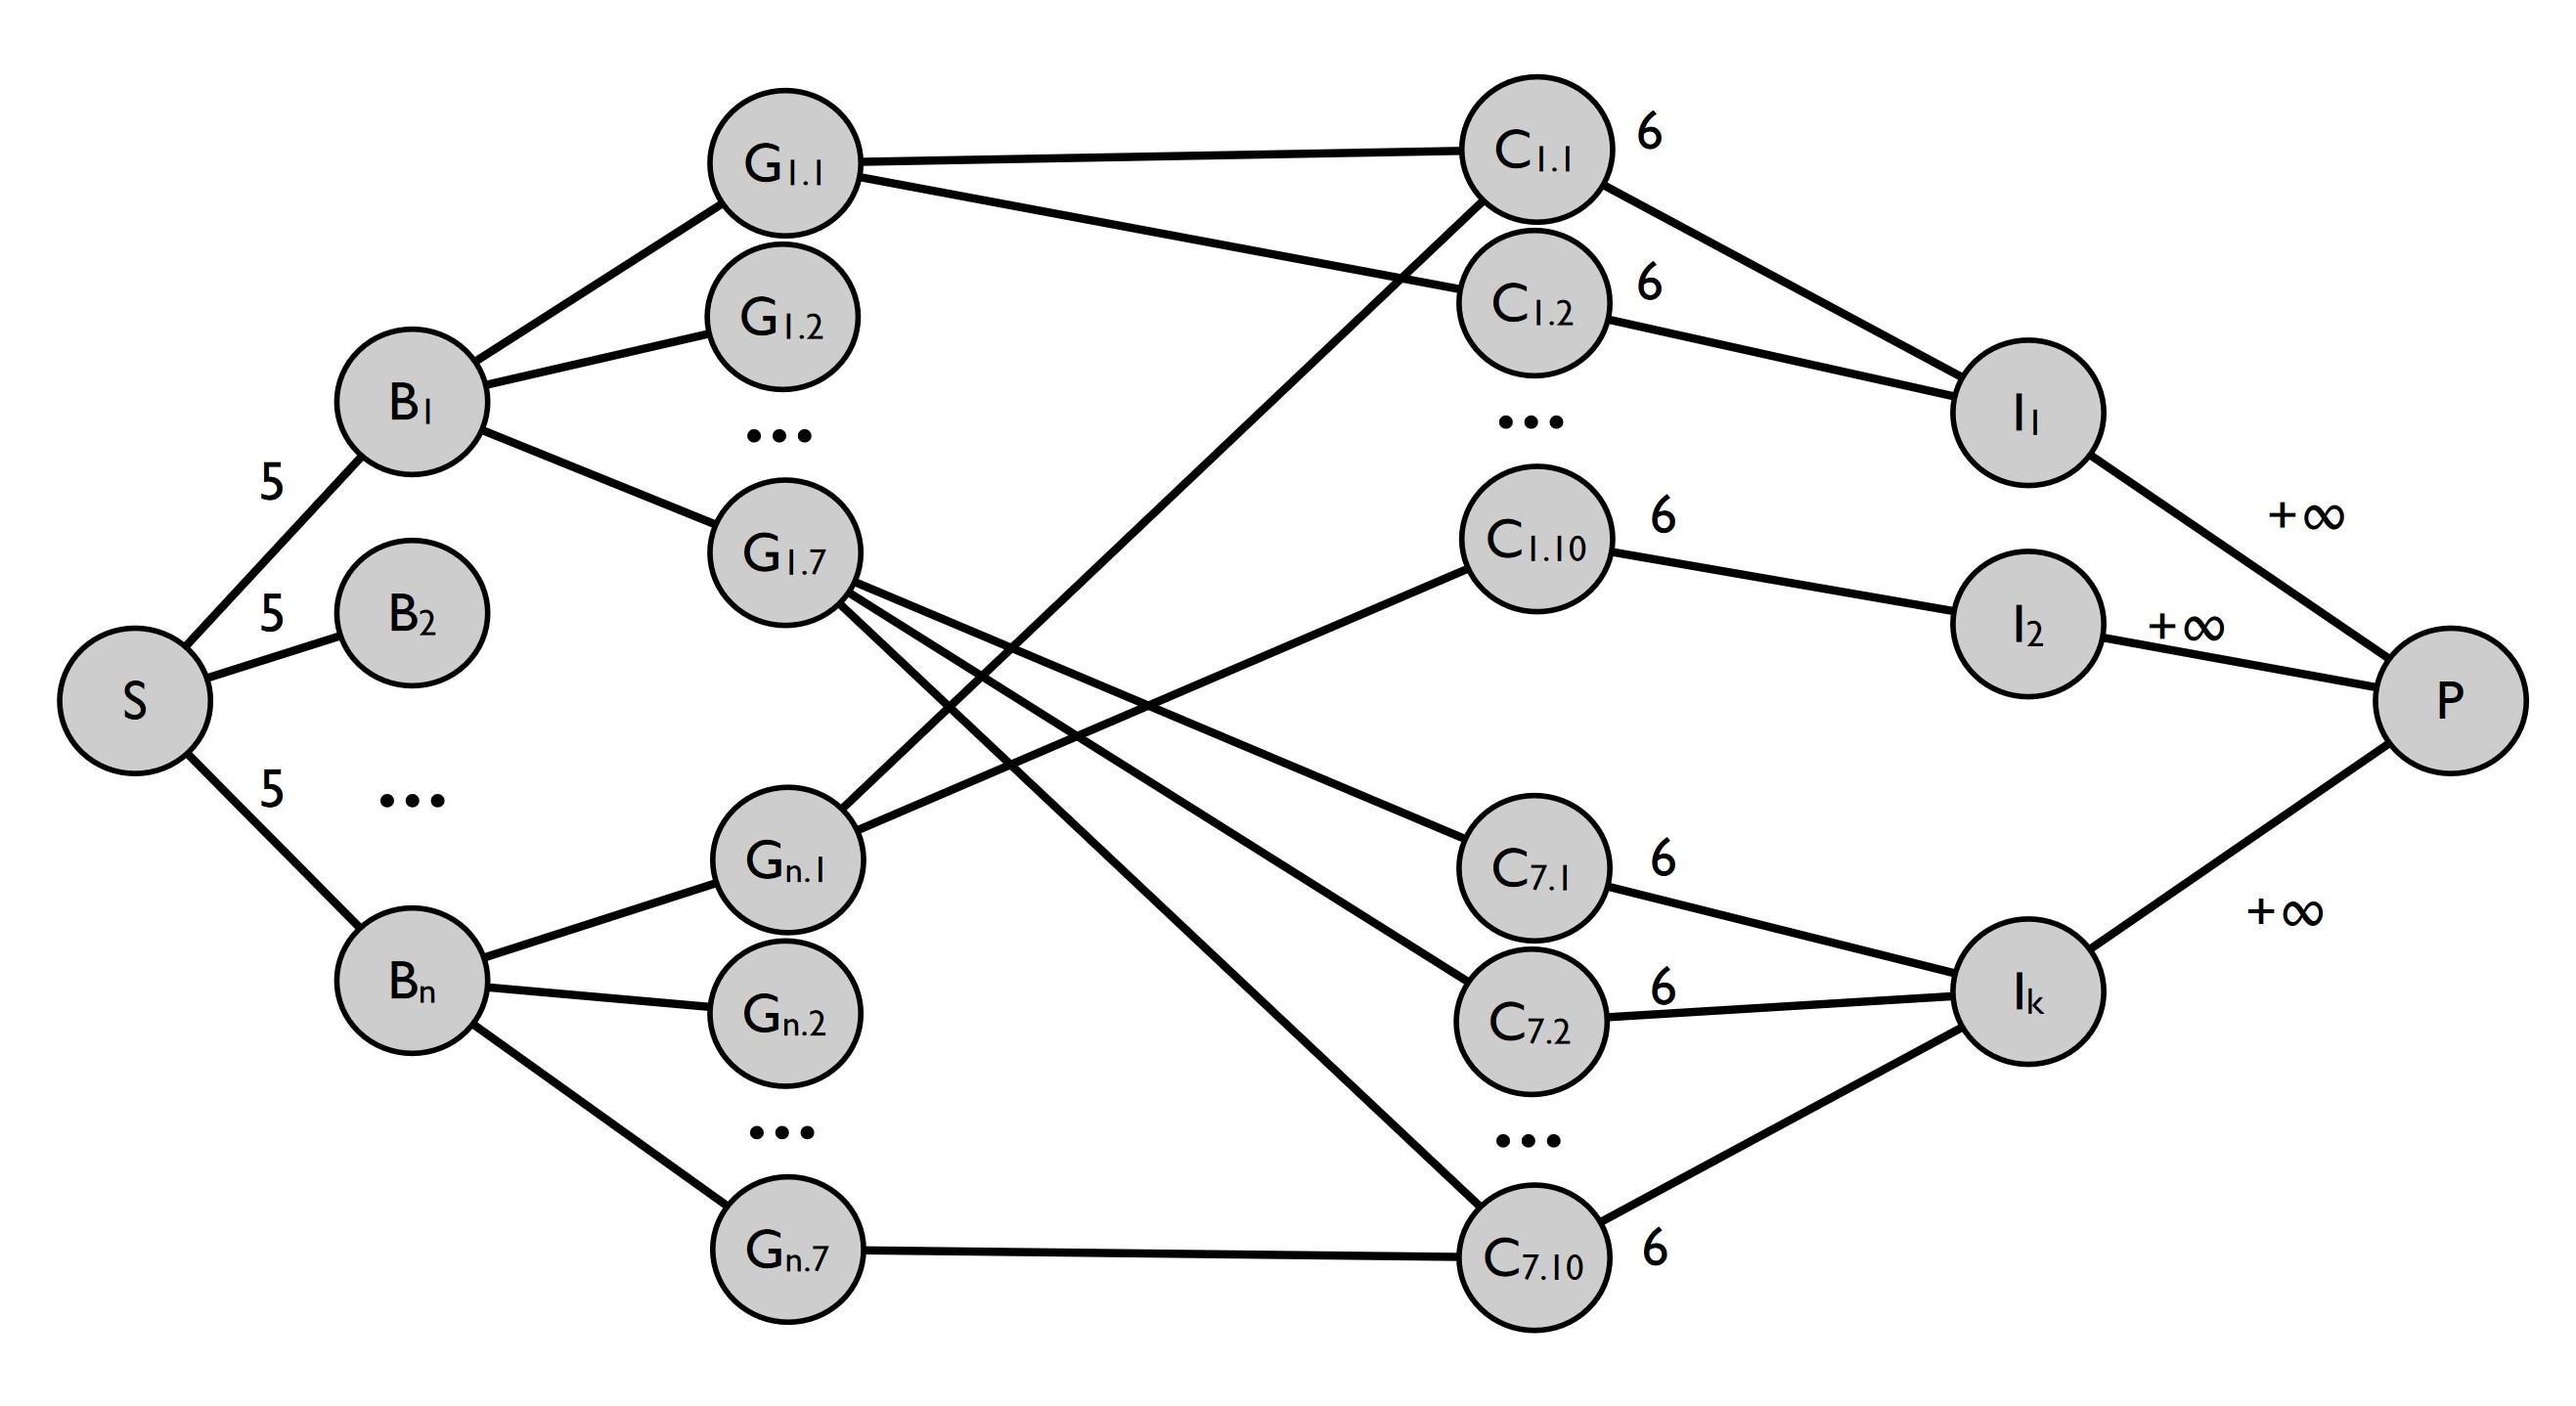
\includegraphics[width=0.7\textwidth]{../img/Locale_5.jpg}
\end{figure}
\newpage
\end{document}